\section{Polygons}

\begin{frame}
  \centering
  {\bf Part III -- Polygons and Convex Hull}

\end{frame}

\begin{frame}[fragile]
  \frametitle{Polygons -- Definition and data structure}

    A polygon is a plane figure bounded by a finite sequence of line
    segments.

  \begin{exampleblock}{Polygon Representation}
    \begin{itemize}
    \item In general, we store an array of points of the segments;
    \item We want to sort the points in CW or CCW order;
    \item Add the first point at the end of the array to avoid
      special cases;
    \end{itemize}
{\smaller
\begin{verbatim}
// 6 points, entered in counter clockwise order;
vector<point> P;
P.push_back(point(1, 1)); // P0
P.push_back(point(3, 3)); // P1
P.push_back(point(9, 1)); // P2
P.push_back(point(12, 4)); // P3
P.push_back(point(9, 7)); // P4
P.push_back(point(1, 7)); // P5
P.push_back(P[0]); // important: loop back
\end{verbatim}}
\end{exampleblock}
\end{frame}

\begin{frame}[fragile]
  \frametitle{Characteristics of a Polygon}
  {\smaller
    \begin{exampleblock}{Perimeter of a Poligon -- add the distances of the segments}
\begin{verbatim}
double perimeter(const vector<point> &P) {
  double result = 0.0;
  for (int i = 0; i < (int)P.size()-1; i++)
     // remember: P[0] = P[P.size()-1]
     result += dist(P[i], P[i+1]);
  return result; }
\end{verbatim}
    \end{exampleblock}

    \begin{exampleblock}{Area of a Poligon -- half of the determinant of the XY matrix of segments}
\begin{verbatim}
double area(const vector<point> &P) {
  double result = 0.0, x1, y1, x2, y2;
  for (int i = 0; i < (int)P.size()-1; i++) {
    x1 = P[i].x; x2 = P[i+1].x;
    y1 = P[i].y; y2 = P[i+1].y;
    result += (x1 * y2 - x2 * y1); }
  return fabs(result) / 2.0; }
\end{verbatim}
    \end{exampleblock}
}
\end{frame}


\begin{frame}[fragile]
  \frametitle{Testing if a Polygon is Convex}
  \begin{itemize}
    \item A convex polygon has no "holes";
    \item For any 2 points $p_1,p_2$ inside the polygon, segment is inside polygon too.
  \end{itemize}

    {\smaller
    \begin{exampleblock}{Easier Convex Testing: Every angle turns the same way}
\begin{verbatim}
bool isConvex(const vector<point> &P) {
  // Returns true if every 3 neighb vertices turn the same way;
  int sz = (int)P.size();
  if (sz <= 3) return false; // Not a polygon

  bool isLeft = ccw(P[0], P[1], P[2]); // described earlier

  for (int i = 1; i < sz-1; i++)
    if (ccw(P[i],P[i+1],P[(i+2) == sz ? 1 : i+2]) != isLeft)
      return false;            // not same direction as isLeft.

  return true;
}
\end{verbatim}
    \end{exampleblock}
  }
\end{frame}

\begin{frame}[fragile]
  \frametitle{Polygon -- Test point inside the polygon}
    % \begin{block}{There are many ways to test if a point $P$ is in a polygon.}
    %   \begin{itemize}
    %   \item \structure{Winding Algorithm}: Sum the angles of all
    %     angles $APB$ ($A,B$) are points in the polygon. If the sum is
    %     $2\pi$. Point is in polygon.
    %   \item \structure{Ray Casting Algorithm}: Draw an segment from
    %     $P$ to infinity, and count the number of polygon edges
    %     crossed. Odds: Inside. Even: Outside.
    %   \end{itemize}
    % \end{block}

  We can use the same idea to test if a point is inside the polygon: The direction of the point in relation to every edge should be the same.

    {\smaller
    \begin{exampleblock}{Winding Algorithm Code for point in polygon detection}
\begin{verbatim}
bool inPolygon(point pt, const vector<point> &P) {
  if ((int)P.size() == 0) return false;
  double sum = 0;

  for (int i = 0; i < (int)P.size()-1; i++) {
    if (ccw(pt, P[i], P[i+1]))
      sum += angle(P[i], pt, P[i+1]);       //left turn/ccw
      else sum -= angle(P[i], pt, P[i+1]);  //right turn/cw
  }

  return fabs(fabs(sum) - 2*PI) < EPS;
}
\end{verbatim}
    \end{exampleblock}
  }

  {\bf QUIZ:} What happens if the point is at an edge segment?
\end{frame}

\begin{frame}[fragile]
  \frametitle{Polygon -- Cutting}
  % TODO: Add an image explaining Polygon cutting
  {\smaller
    \begin{block}{}
      To cut $P$ along a line $AB$, we separate the points in $P$ to the
      left and right of the line.
    \end{block}

{\smaller
    \begin{exampleblock}{}
\begin{verbatim}
point lineIntersectSeg(point p, point q, point A, point B) {
  double a = B.y-A.y; double b = A.x - B.x; double c = B.x*A.y - A.x*B.y;
  double u = fabs(a*p.x + b*p.y + c); double v = fabs(a*q.x + b*q.y + c);
  return point((p.x*v + q.x*u)/(u+v), (p.y*v + q.y*u)/(u+v)); }

vector<point> cutPolygon(point a, point b, const vector<point> &Q){
  vector<point> P;
  for (int i = 0; i < (int)Q.size(); i++) {
    double left1 = cross(toVec(a, b), toVec(a, Q[i])), left2 = 0;
    if (i != (int)Q.size()-1)
      left2 = cross(toVec(a, b), toVec(a, Q[i+1]));
    if (left1 > -EPS)
      P.push_back(Q[i]);                            //Q[i] is on the left of ab
    if (left1*left2 < -EPS)                         //edge (Q[i], Q[i+1]) crosses line ab
      P.push_back(lineIntersectSeg(Q[i], Q[i+1], a, b)); }
  if (!P.empty() && !(P.back() == P.front()))
    P.push_back(P.front());                         // make P's first point = P's last point
  return P; }
\end{verbatim}
    \end{exampleblock}}
  }
\end{frame}

\begin{frame}
  \frametitle{Polygon -- Convex Hull}

  \begin{itemize}
    \item A common problem: Given a set of points $S$, what is the {\bf smallest convex polygon} that includes all points in $S$?\bigskip

    \item One way to find the Convex Hull: for each point $p \in S$, determine if the point is at the edge of the polygon (in the hull) or inside the polygon (not in the hull).\bigskip

    \item We will introduce the $O(n\log n)$ algorithm "Graham's Scan"
  \end{itemize}

    \begin{center}
      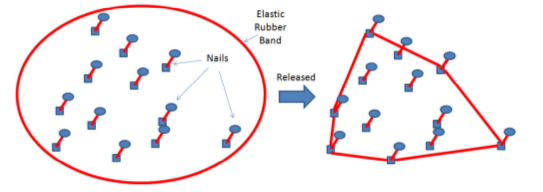
\includegraphics[width=.7\textwidth]{../img/convexhull_halim}
      \ppagenote{Convex Hull image by Steven Halim "Competitive Programming 3"}
    \end{center}
\end{frame}

\begin{frame}[fragile]
  \frametitle{Polygon -- Graham's Scan}
  \framesubtitle{Helper Functions -- sort two points based on their angle against the X axis}

{\small
\begin{exampleblock}{}
\begin{verbatim}
point pivot(0, 0);

bool angleCmp(point a, point b) {
  // special case: if collinear, choose closet to pivot;
  if (collinear(pivot, a, b)) // special case
    return dist(pivot, a) < dist(pivot, b);

  // calculate angle against the X axis:
  double d1x = a.x - pivot.x, d1y = a.y - pivot.y;
  double d2x = b.x - pivot.x, d2y = b.y - pivot.y;

  return (atan2(d1y, d1x) - atan2(d2y, d2x)) < 0;
}
\end{verbatim}
\end{exampleblock}
}
\end{frame}

\begin{frame}[fragile]
  \frametitle{Polygon -- Graham's Scan}
  \framesubtitle{Convex Hull -- Initializing the algorithm}

  {\small
    \begin{exampleblock}{}
\begin{verbatim}
vector<point> CH(vector<point> P) {
  int i, j, n = (int)P.size();
  // Special Case: Polygon with 3 points
  if (n <= 3) {
    if (!(P[0]==P[n-1])) P.push_back(P[0]);
    return P; }

  // Find Initial Point: Low Y then Right X
  int P0 = 0;
  for (i = 1; i < n; i++)
    if (P[i].y < P[P0].y ||
        (P[i].y == P[P0].y && P[i].x > P[P0].x))
      P0 = i;
  point temp = P[0]; P[0] = P[P0]; P[P0] = temp;
\end{verbatim}
\end{exampleblock}}
\end{frame}

\begin{frame}[fragile]
  \frametitle{Polygon -- Graham's Scan}
  \framesubtitle{Convex Hull -- More initialization}
  {\small
    \begin{exampleblock}{}

\begin{verbatim}

  // second, sort points by angle with pivot P0
  pivot = P[0];
  sort(++P.begin(), P.end(), angleCmp);

  // S holds the Convex Hull
  // We initialize it with first three points
  vector<point> S;
  S.push_back(P[n-1]);
  S.push_back(P[0]);
  S.push_back(P[1]);

  // We start on the third point
  i = 2;
\end{verbatim}

    \end{exampleblock}
  }
\end{frame}

\begin{frame}[fragile]
  \frametitle{Polygon -- Graham's Scan}
  \framesubtitle{Convex Hull -- Main Loop}

Now that we selected a pivot and sorted the points, we test every three points (following the sort) if they are in the convex hull.

  {\small
    \begin{exampleblock}{}
\begin{verbatim}
  while (i < n) {
    j = (int) S.size() - 1;
    // If the next point is left of CH, keep it.
    // Else, pop the last CH point and try again.

    if (ccw(S[j-1], S[j], P[i]))
      S.push_back(P[i++]);
    else
      S.pop_back();
    }
  return S;
}                 // End Graham's Scan CH
\end{verbatim}
\end{exampleblock}}
\end{frame}
%% TODO: Add polygon problem example
